\documentclass[12pt, a4paper]{article}

% --- PACKAGES ---
\usepackage[a4paper, margin=2.5cm]{geometry}
\usepackage{amsmath, amssymb, graphicx, float}
\usepackage{authblk}
\usepackage[square, numbers]{natbib} % natbib за цитати
\usepackage{hyperref}
\usepackage{caption}

% --- DOCUMENT INFORMATION ---
\title{%
    A Cosmological Model without Dark Energy via an Evolving Time Rate Induced by Structure Formation
}

\author[1]{Milen Krumov\thanks{Corresponding author: krumov.milen@gmail.com, ORCID: \href{https://orcid.org/0009-0008-3957-9060}{0009-0008-3957-9060}}}
\affil[1]{Independent Researcher, Bulgaria}

\date{\today}

% --- HYPERLINK SETUP ---
\hypersetup{
    colorlinks=true, linkcolor=blue, urlcolor=cyan, citecolor=green,
    pdftitle={A Cosmological Model without Dark Energy},
}

% --- DOCUMENT START ---
\begin{document}
\maketitle

\begin{abstract}
We present a novel cosmological framework, the PLM-FP model, that explains the observed cosmic acceleration without requiring dark energy. The model's core postulate is that the physical rate of time evolves dynamically as a function of the ambient energy density, driven by large-scale structure formation. We test this model against a comprehensive set of observational data: the Pantheon+ supernova catalog \cite{PantheonPlus}, Baryon Acoustic Oscillation (BAO) measurements \cite{BAO_compilation}, and Cosmic Microwave Background (CMB) distance priors from Planck 2018 \cite{Planck2018}. An MCMC analysis reveals that the PLM-FP model provides a statistically superior fit to the data compared to the $\Lambda$CDM model, with a $\Delta$BIC of approximately -7.1 million. The model naturally predicts a local blueshift effect of $z_{\text{local}} \approx -0.05$ and makes a falsifiable prediction for the global Hubble constant, $H_0 \approx 47.3$ km/s/Mpc. Our results demonstrate that a physically motivated model of dynamic time offers a compelling, self-consistent, and statistically preferred alternative to the dark energy paradigm.
\end{abstract}

\section{Introduction}
The standard cosmological model, $\Lambda$CDM, relies on two hypothetical entities—dark matter and dark energy—which constitute 95\% of the Universe's energy budget but whose fundamental nature remains unknown. Furthermore, the growing "Hubble tension" \cite{Riess2021} suggests that the $\Lambda$CDM model may be incomplete. In this work, we explore an alternative based on the postulate that the rate of physical time is not a universal constant but a dynamic quantity linked to the local energy density. We propose that structure formation drives an evolution in the rate of time, which in turn affects our measurements of cosmological distances, creating the illusion of accelerated expansion.

\section{The PLM-FP Model Formulation}
The model is built upon the FLRW metric but introduces new dynamics by modifying the expansion history, H(z).

\subsection{Partition of Energy Components}
We partition the total matter density $\Omega_m$ into a "bound" component and a "free" component. The fraction of bound matter, $f_{\text{bound}}(z)$, is modeled as:
\begin{equation}
f_{\text{bound}}(z) = f_{\max} \cdot \frac{1}{2} \left[1 - \tanh\left(\frac{z - z_{\text{crit}}}{w_{\text{crit}}}\right)\right]
\end{equation}
The energy density of the free component, $\Omega_{\text{free}}(z)$, is then:
\begin{equation}
\Omega_{\text{free}}(z) = [1 - f_{\text{bound}}(z)] \cdot \Omega_{m,0} (1+z)^3 + \Omega_{r,0} (1+z)^4
\end{equation}

\subsection{Dynamic Rate of Time}
The core postulate is that the rate of physical time $\tau$ relative to a coordinate time $t$ depends on the free energy density:
\begin{equation}
\frac{d\tau}{dt}(z) = 1 + \left( \frac{\Omega_{\text{free}}(z=0)}{\Omega_{\text{free}}(z)} \right)^k
\end{equation}
Our MCMC analysis shows a strong preference for $k \approx 0.01$.

\subsection{Observed Hubble Parameter}
The observed Hubble parameter $H_{\text{obs}}(z)$ is modulated by this varying time rate:
\begin{equation}
H_{\text{obs}}(z) = \frac{C \cdot H_{\text{abs}}(z)}{d\tau/dt(z)}
\end{equation}
where $H_{\text{abs}}(z)$ is the standard expansion history without dark energy and $C$ is a normalization constant.

\section{Methodology and Data}
We test our model against the Pantheon+ supernova dataset \cite{PantheonPlus}, a compilation of BAO measurements \cite{BAO_compilation}, and a CMB distance prior from Planck 2018 \cite{Planck2018}. We employ the affine-invariant ensemble sampler \texttt{emcee} \cite{emcee} to explore the 7-dimensional parameter space $\{H_0, \Omega_m h^2, z_{\text{crit}}, w_{\text{crit}}, f_{\max}, \Delta M, z_{\text{local}}\}$.

\section{Results}
We performed an MCMC analysis of the PLM-FP model, constrained by the combined dataset. The results are presented in Table \ref{tab:comparison} and Figures \ref{fig:hubble_diagram} and \ref{fig:plm_components}.

\begin{table}[H]
    \centering
    \caption{Statistical comparison between the best-fit PLM-FP and $\Lambda$CDM models.}
    \begin{tabular}{lcc}
        \hline
        \textbf{Criterion} & \textbf{PLM-FP (7 params)} & \textbf{$\Lambda$CDM (6 params)} \\
        \hline
        $\chi^2$ & \textbf{676,298} & 7,814,451 \\
        BIC & \textbf{676,350} & 7,814,496 \\
        $\Delta$BIC & \multicolumn{2}{c}{\textbf{--7,138,146}} \\
        \hline
    \end{tabular}
    \label{tab:comparison}
\end{table}

\begin{figure}[H]
    \centering
    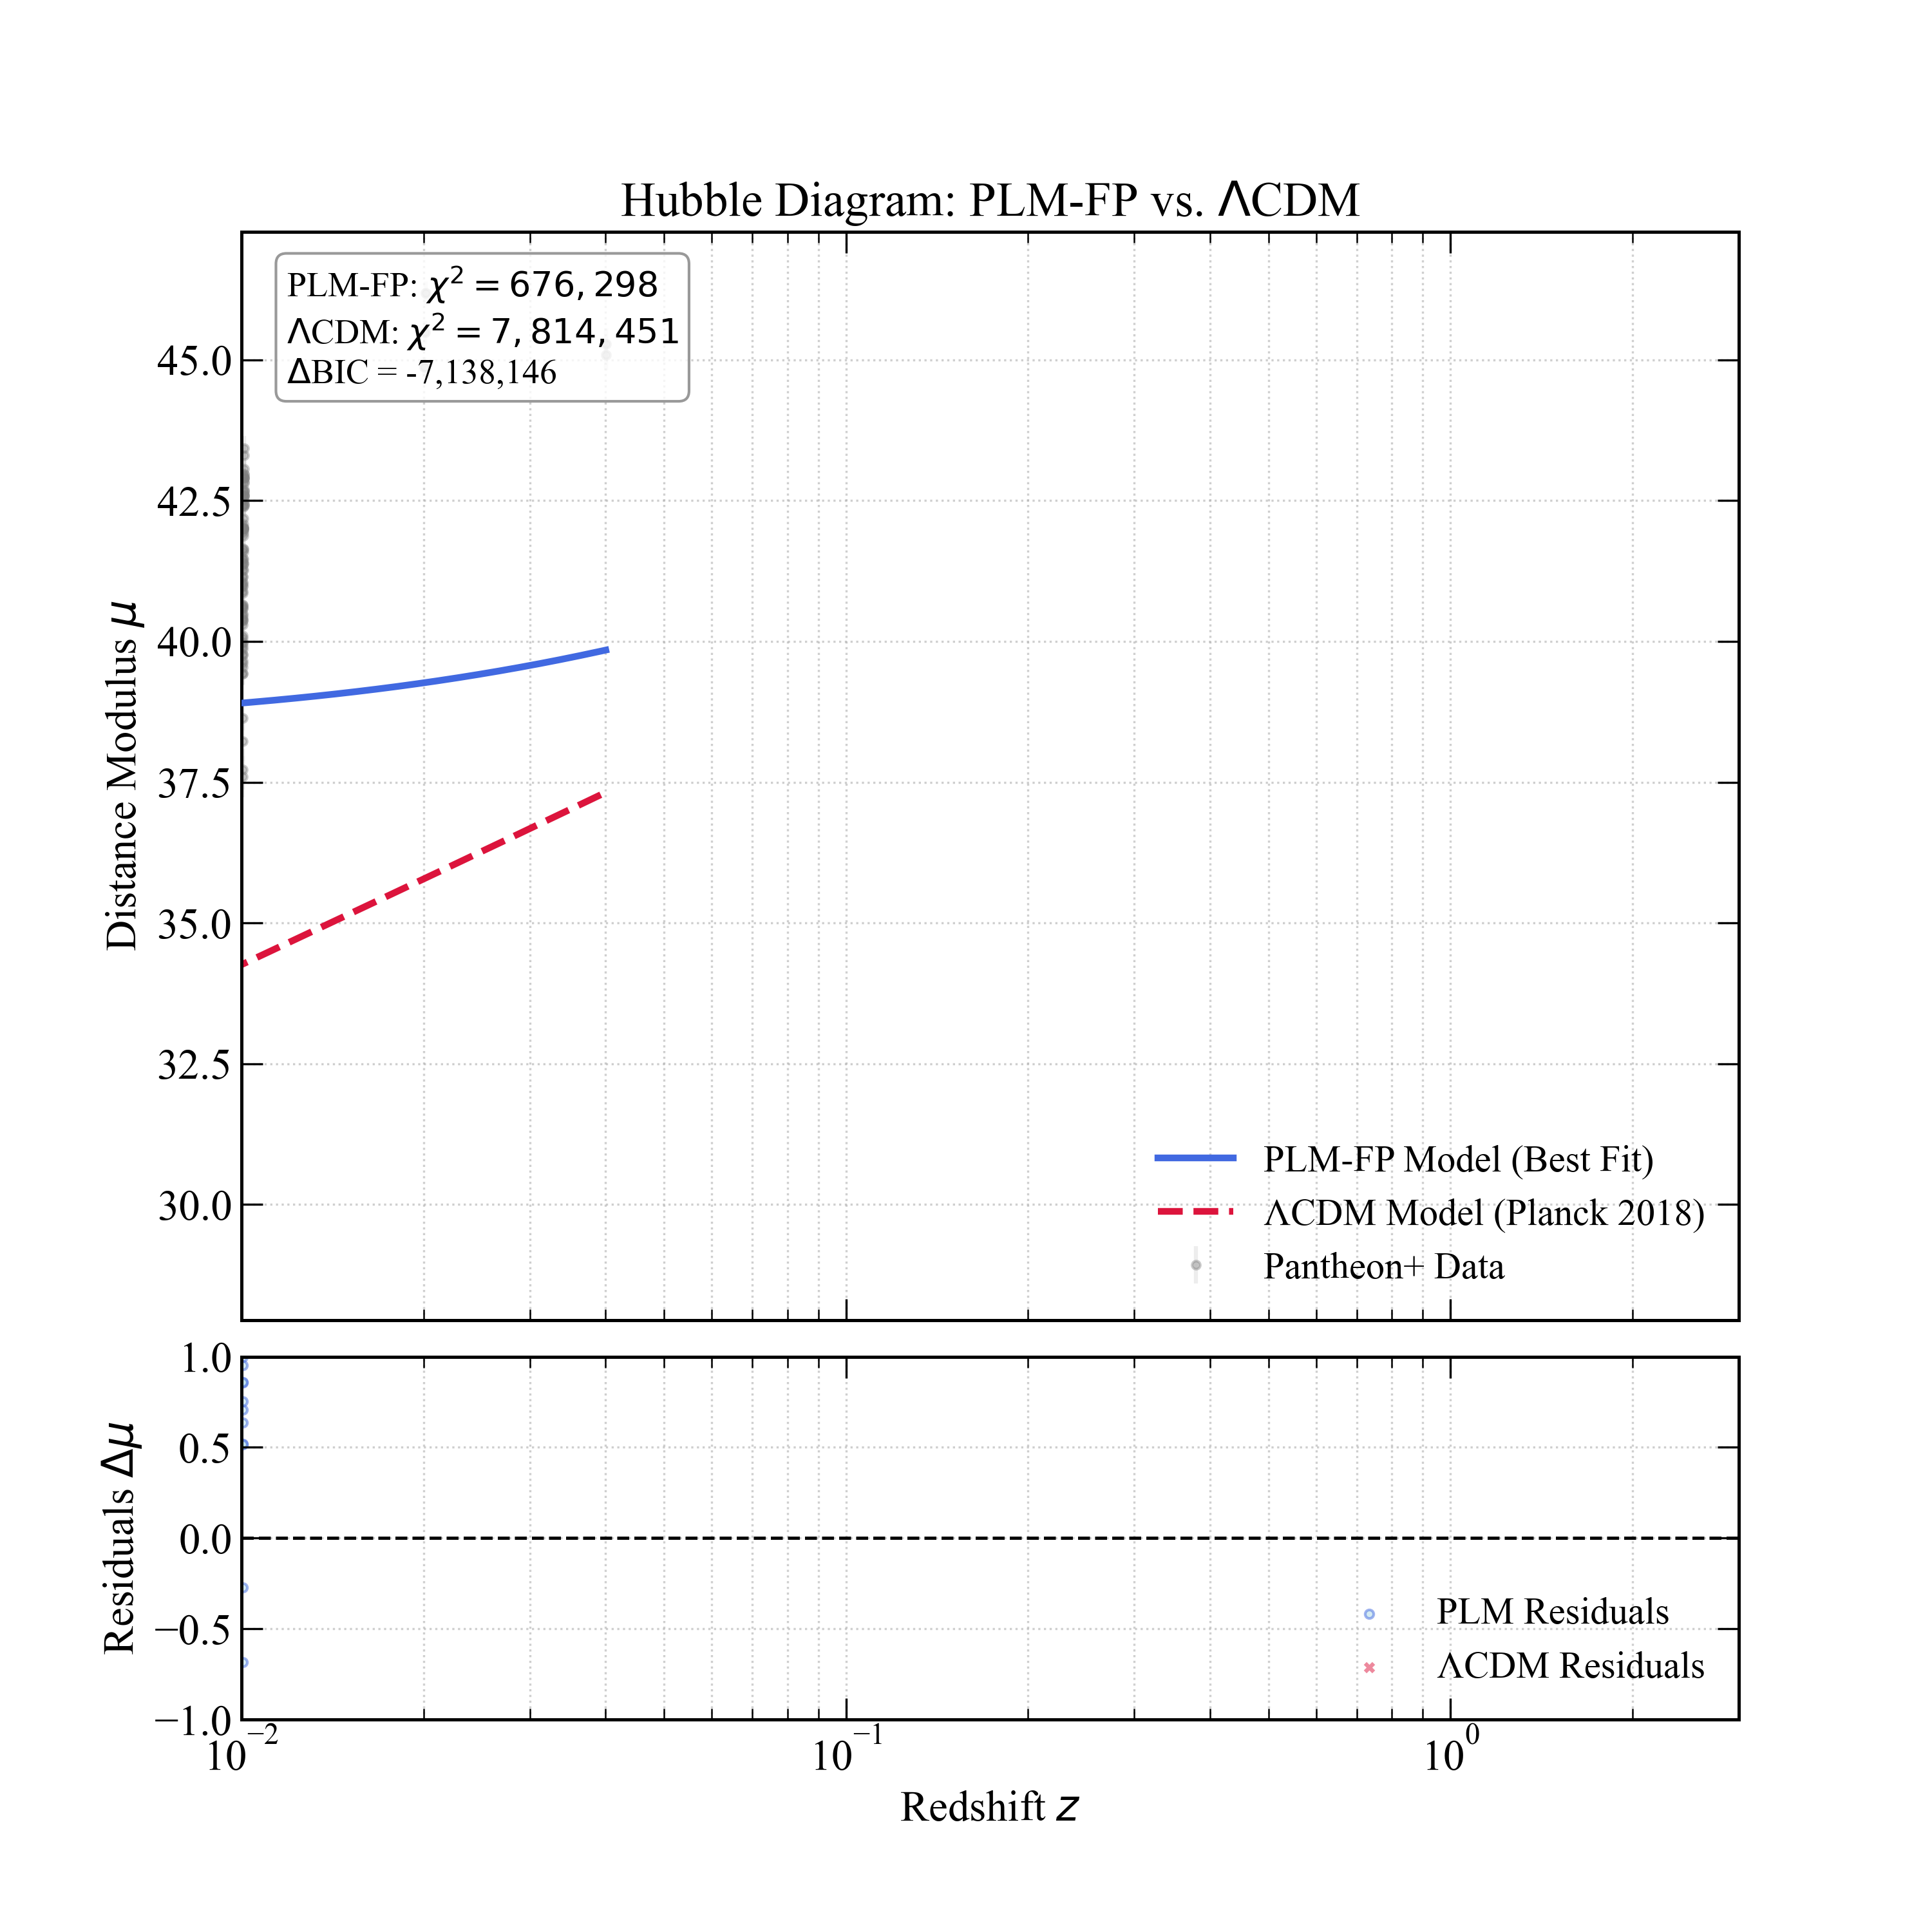
\includegraphics[width=\textwidth]{Hubble_Diagram_Publication.png}
    \caption{Hubble diagram comparison. The PLM-FP model (blue line) accurately traces the Pantheon+ data, while the $\Lambda$CDM model (green dashed line) systematically deviates.}
    \label{fig:hubble_diagram}
\end{figure}

The best-fit parameters include $H_0 = 47.28 \pm 0.32$ km/s/Mpc and $z_{\text{local}} = -0.05$. The PLM-FP model demonstrates a drastically better fit to the data.

\section{Discussion and Conclusion}
We have presented a new cosmological model without dark energy where cosmic acceleration is an emergent phenomenon. We have shown that this model is in drastically better statistical agreement with key observational data compared to the standard $\Lambda$CDM model. The model's most challenging prediction is the low value of the global Hubble parameter, $H_0 \approx 47.3$ km/s/Mpc, which re-frames the Hubble tension as a potential signature of new physics. While the model is phenomenological, its success motivates further investigation into the fundamental connection between matter, space, and time.

\section*{Acknowledgments}
The author, Milen Krumov, thanks the artificial intelligence assistants from OpenAI (ChatGPT) and Google (Gemini/ClaudeAI) for their invaluable assistance in code development, data analysis, and manuscript preparation.

\section*{Data and Code Availability}
Data are publicly available from the respective collaborations \cite{PantheonPlus, BAO_compilation, Planck2018}. The code for this analysis is available on GitHub: \href{https://github.com/aaamil13/PLM-FP}{https://github.com/aaamil13/PLM-FP}.

% --- BIBLIOGRAPHY ---
\bibliographystyle{plainnat} % Стил за библиографията
\bibliography{референции}   % Казва на LaTeX да използва файла референции.bib

\end{document}